% !TeX program = latexmk
% !TeX spellcheck = pl_PL
% !TeX root = example.tex

\chapter{Najczęściej wykorzystywane narzędzia w zarzadzaniu projektami.}

Zarządzanie projektami informatycznymi ściśle wiąże się z wykorzystaniem narzędzi informatycznych, które wspomagają ten proces. Przy ich wyborze warto pamiętać, iż mają pomagać w pracy projektowej, a nie przeszkadzać w jej realizacji, dlatego należy wybierać je mądrze. Przykładem nieodpowiedniego doboru narzędzia może być sytuacja, w której kierownik projektu nie dotrzymuje terminów swoich prac, ze względu na zajmowanie się raportowaniem postępu prac lub aktualizacją harmonogramu.\cite{Kopczewski_2015}

\section{Narzędzia stosowane dla metod klasycznych.}

\subsection{Microsoft Project}

Najbardziej popularnym narzędziem stosowanym w metodykach klasycznych jest Microsoft Project. Pozwala on na rozpisanie całego harmonogramu działań, zaplanowanie budżetu czy stworzenie wykresu Gantta, tak niezbędnego w pracy kierownika. Pozwala także na tworzenie raportów, prezentacji i wykresów z postępów prac.\ref{rys:project}

\subsection{Gantt Project}

W niektórych przedsiębiorstwach w zarządzaniu projektami używa się programu Gantt Project. Jest to darmowe narzędzie umożliwiające dynamiczne tworzenie diagramów Gantta z podziałem na poszczególne zadania wraz z rozplanowaniem ich w czasie. Dodatkowo pozwala ono na tworzenie wykresów PERT (ang. Program Evaluation and Review Technique) wraz ze ścieżkami krytycznymi.\cite{Trendy_Zarzadzanie}

\begin{figure}
	\centering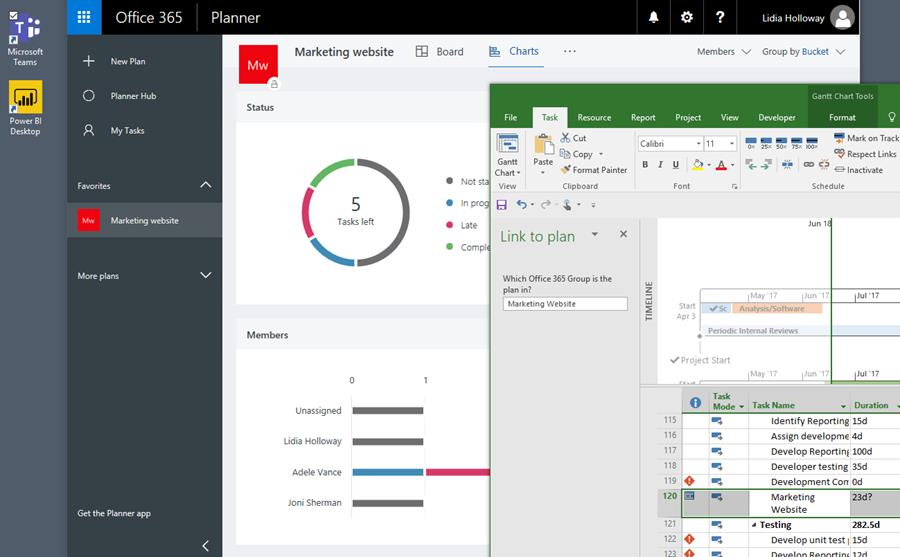
\includegraphics[width=.6\textwidth]{img/Microsoft_Project}
	\caption{Microsoft Project[www.microsoft.com]} \label{rys:project}% Źródło rysunku i etykieta przez którą odwołujemy się do rysunku.
\end{figure}

\newpage

\section{Najpopularniejsze narzędzia stosowane dla metod zwinnych ( team estimation game, kanban, planning poker).}

W małych zespołach projektowych, które wykorzystują metodyki zwinne, odchodzi się zazwyczaj od Microsoft Project czy GanttProject stosując aplikacje webowe. Przykładem takich aplikacji są: Jira, Mantis, TFS, Trello, Sllack, KanbanTool. 
Przy metodykach zwinnych, właściciel produktu tworzy rejestr produktowy (ang. Product Backlog), który ma formę listy zawierającej wymagania klienta z określoną wagą  (priorytetem) i czasochłonnością.\cite{Shwaber_2004} Wymienione wyżej narzędzia pozwalają na taką pracę i umieszczanie danych w chmurze, dzięki czemu każdy członek zespołu ma do nich dostęp, niezależnie od lokalizacji, czy pracuje w biurze czy poza nim. Zadania w backlogu\footnote{Backlog – rejestr sprintu / lista zadań\cite{metody_zwinne_2016}} powinny być rozpisane dla obecnego sprintu \footnote{Sprint – jeden z etapów niektórych metodyk zwinnych, który wyznacza rytm pracy. W jego
trakcie następuje faktyczne wykonanie określonej funkcjonalności\cite{Samoorganizacja_2010}} oraz zawierać dodatkowe zadania, które będą zasilać kolejny sprint bądź zostaną wykonane w istniejącym, gdy nadarzy się taka możliwość. Takie odejście do pracy umożliwia wykonanie części zadań przed wyznaczonym czasem. Narzędzia te pozwalają również na przypisanie konkretnego zadania do danego użytkownika, dzięki czemu każdy pracownik zna zakres swojej odpowiedzialności; takie rozwiązanie zapobiega wykonaniu tego samego zadania przez kilka osób.
Niektóre firmy, a można nawet powiedzieć, że wiele firm, niezależnie od wykorzystywanej metodyki używa Microsoft Excela do zarządzania projektami (przyzwyczajenia?). Umożliwia on przedstawienie danych w postaci tabeli oraz różnych grafów. Każda firma może zarządzać nim na swój własny sposób, dzięki czemu proces ten jest bardzo elastyczny. Ponadto ułatwia on wykonanie prognoz przyszłych dochodów, kalkulacji wybranych parametrów i wskaźników. Kolejnym narzędziem wykorzystywanym na szeroką skalę jest SharePoint, który umożliwia współdzielenie plików czy tworzenie listy zadań, która może być wykorzystana w MS Project.

Przejdźmy wreszcie do narzędzi stosowanych w metodach zwinnych. Bardzo często w projektach zwinnych planujemy bez użycia dni i godzin. W klasycznych projektach tworzymy harmonogramy, szczegółowe plany, gdzie mamy daty, gdzie mamy godziny, gdzie każde zadanie ma określony czas realizacji. W przypadku projektów zwinnych często odchodzimy od tak szczegółowego planowania, ale jakaś forma planowania oczywiście jest potrzebna, dlatego stosujemy różne alternatywne metody i jedną z takich alternatywnych metod jest metoda nazwana Team Estimation Game.


\section{Odniesienie do książki}

Jak pisze Harel w \cite{harel_rzecz_2008}: \lipsum[7]


\subsection{Rysunek z kotem}

Jak widać na rys.\ref{rysunek:kot} Ala ma kota. \lipsum[9-10] 

\begin{figure}
\centering
\includegraphics[width=.4\textwidth]{img/kotek}
\caption{Ala ma kota (opr.wł).}\label{rysunek:kot}
\end{figure}

\subsection{Tabela}

Co uwzględniono w tabeli \ref{tabela:coktoma}. \lipsum[13-15] 

% Tabela. Nazwa tabeli u góry.
\begin{table}
\centering\caption{Co kto ma \cite{harel_rzecz_2008} (patrz też dodatek~\ref{Dod1}) \label{tabela:coktoma}}
\begin{tabular}{|l|l|l|}% wyrównanie kolumn tabeli -> l c r - do lewej, środka, do prawej
\hline
Ala & ma & kota \\
\hline
Ola & ma & psa \\
\hline
Ula & ma & małpę\\
\hline
\end{tabular}
\end{table}

\lipsum[19-20] Warto wspomnieć, że w \cite{aizawa_groundwater_2009} rzecz przedstawiona jest zupełnie inaczej. Poniższy wzór:

\begin{equation}
\sum_{i=1}^{\infty}a_i
\label{eq:mojWzor}
\end{equation}

Wzór \ref{eq:mojWzor} wskazuje że dowód podany w \cite{kaleta_experimental_2005} może zostać podważony. \lipsum[9]

\section{Listing}

% lub {java} albo {bash} albo {text}
\begin{listing}
\begin{minted}{c} 
int main()
{
   int a=2*3;
   printf("**Ala ma kota\n**");
   while(!I2C_CheckEvent(I2C1, I2C_EVENT_MASTER_MODE_SELECT)); /* EV5 */
   return 0;
}
\end{minted}
\caption{Przykładowy algorytm w języku C (opr. wł.)} \label{listing:moj}
\end{listing}

W moim kodzie \ref{listing:moj} zrobiłem coś wspaniałego. \lipsum[4]
